\justify
\skipspace

This is going to be more of a summary and some implementation details of my first ever experience with computer graphics and making games.

Two weeks ago, not knowing anything about computer graphics and game development, I embarked on a journey down the rabbit hole of creating one of the pioneering games of video game history, such as the OG \textit{Doom} and \textit{Wolfenstein 3D}.

I decided to create a raycasting engine in \textit{C++} using the \textit{Simple DirectMedia Layer} graphics library. And for a beginner like me, it was quite the challenge.

The whole idea of making this in a very bare-bones library and language like \textit{SDL2} and \textit{C++} was because I wanted to create something that would be truly cross-platform from the start. And by cross-platform I mean \textbf{cross-platform}. The game would run on all desktop operating systems (Linux, Windows, Apple) and all mobile operating systems (Android, iOS, Raspberry Pi, Chrome)! And of course the \textsc{PSP}. I could talk a lot about why the PSP, but I'll save that for another time.

\section*{Introduction}

Now you must be asking - "Bruh, what even is a Raycaster".

The simplest way to explain it is that it's a rendering technique to create a 3D perspective from a 2D map, what we like to call as 2.5D.

Although this is about the making of a raycasting game engine, I had to give a lot of thought on how game engines are structured in the first place.

I wanted my project to follow the \textit{Object-Oriented} design pattern as well so that it would be easy to extend and plug in components without touching a lot of code, enabling a deeper level of abstraction. I taught me a lot about inheritance and composition in C++.

\section*{The Game Engine}

I'll talk about the game architecture in this section.

The engine was written in C++ and then compiled using the \textit{CMake} build system, which enables me to go completely cross-platform.

The high level architecture of the engine
looks something like this:\\[1cm]


\begin{tikzpicture}[
    node distance = 8mm and 12mm,
    start chain = A going below,
    arr/.style = {-{Triangle[length=3mm, width=6mm]}, line width= 2mm,
    draw=blue2, shorten > = 1mm, shorten <=1mm},
    base/.style = {draw, semithick, minimum height=12mm, text width=44mm,
            align=flush center},
    BC/.style args = {#1/#2/#3}{
            decorate,
            decoration={calligraphic brace, amplitude=6pt,
                    pre =moveto, pre  length=1pt,
                    post=moveto, post length=1pt,
                    raise=#1,
                    #2},% for mirroring of brace
            very thick,
            pen colour={#3} },
    M/.style = {base, fill=#1,
            tape,
            tape bend top=none, tape bend height=2mm, tape bend bottom=in and out},
    N/.style = {base, rounded corners, fill=#1}
    ]
    % main branch
    \begin{scope}[nodes={on chain=A, join=by arr},
            N/.default=blue2]
        \node [N=blue1]     {Hi};                   % A-1
        \node [N=orange1]   {Hello};    % A-2
        \node [N]   {Hola};
        \node [N]   {He};

    \end{scope}
    % nodes on the left side of the main branch
    \node [N=gray1,
        left=of A-1]     (B-1)   {ACTEURS};
    \coordinate (aux1) at ($(A-3.south west)!0.5!(A-4.north west)$);
    \node [N=gray2,
        left=of aux1]     (B-2)   {Client};

    % nodes on the right side of thr main branch
    \begin{scope}[M/.default=yellow1]
        \node [M, right=of A-2, text width=1cm] (D-1) {C++};
    \end{scope}
\end{tikzpicture}


\section*{Raycasting}

What actually distinguishes my project from any other implementation that you may find on the web is the fact that instead of dividing the whole world into square grids, it defines all the objects and texture rendering using their actual coordinates.

Looking back, using the 2D grid approach while being a lot easier to implement, it's also quite a bit more efficient and accurate.

Having said that, it also restricts a lot of what can be actually created in the game.


The biggest leap of faith I took for this engine was to create the raycasting logic. So, here's how raycasting actually works.

We first need to define these terms:

\begin{itemize}

    \item \textbf{Player direction $\alpha$ :} The direction that the player is currently facing.
    \item \textbf{Maximum view distance $d$ :} The position of the player in the world.
    \item \textbf{Horizontal field of view $\Omega$ :} The visible field of view the player sees in the horizontal direction. I assumed this to be, 100°.
    \item \textbf{Vertical field of view :} This gives an idea of how high or low can the person see. I assume this to be, 60°.
    \item \textbf{Number of rays :} This is the number of rays that we cast from the player's position. You can set this number a lot of ways, and how high you set this will determine how accurate the raycasting will be.

\end{itemize}

\pagebreak

Now we are ready to tackle the actual casting of rays. What our aim is to cast a ray from the player's position in the direction of the player's direction $\alpha$ and then check if it intersects with any of the walls in the map. If it does, then we need to calculate the distance between the player and the wall and then draw a slice of the player's view corresponding to that ray.

So, consider this diagram of the player's situation:

\begin{figure}[!ht]
    \centering
    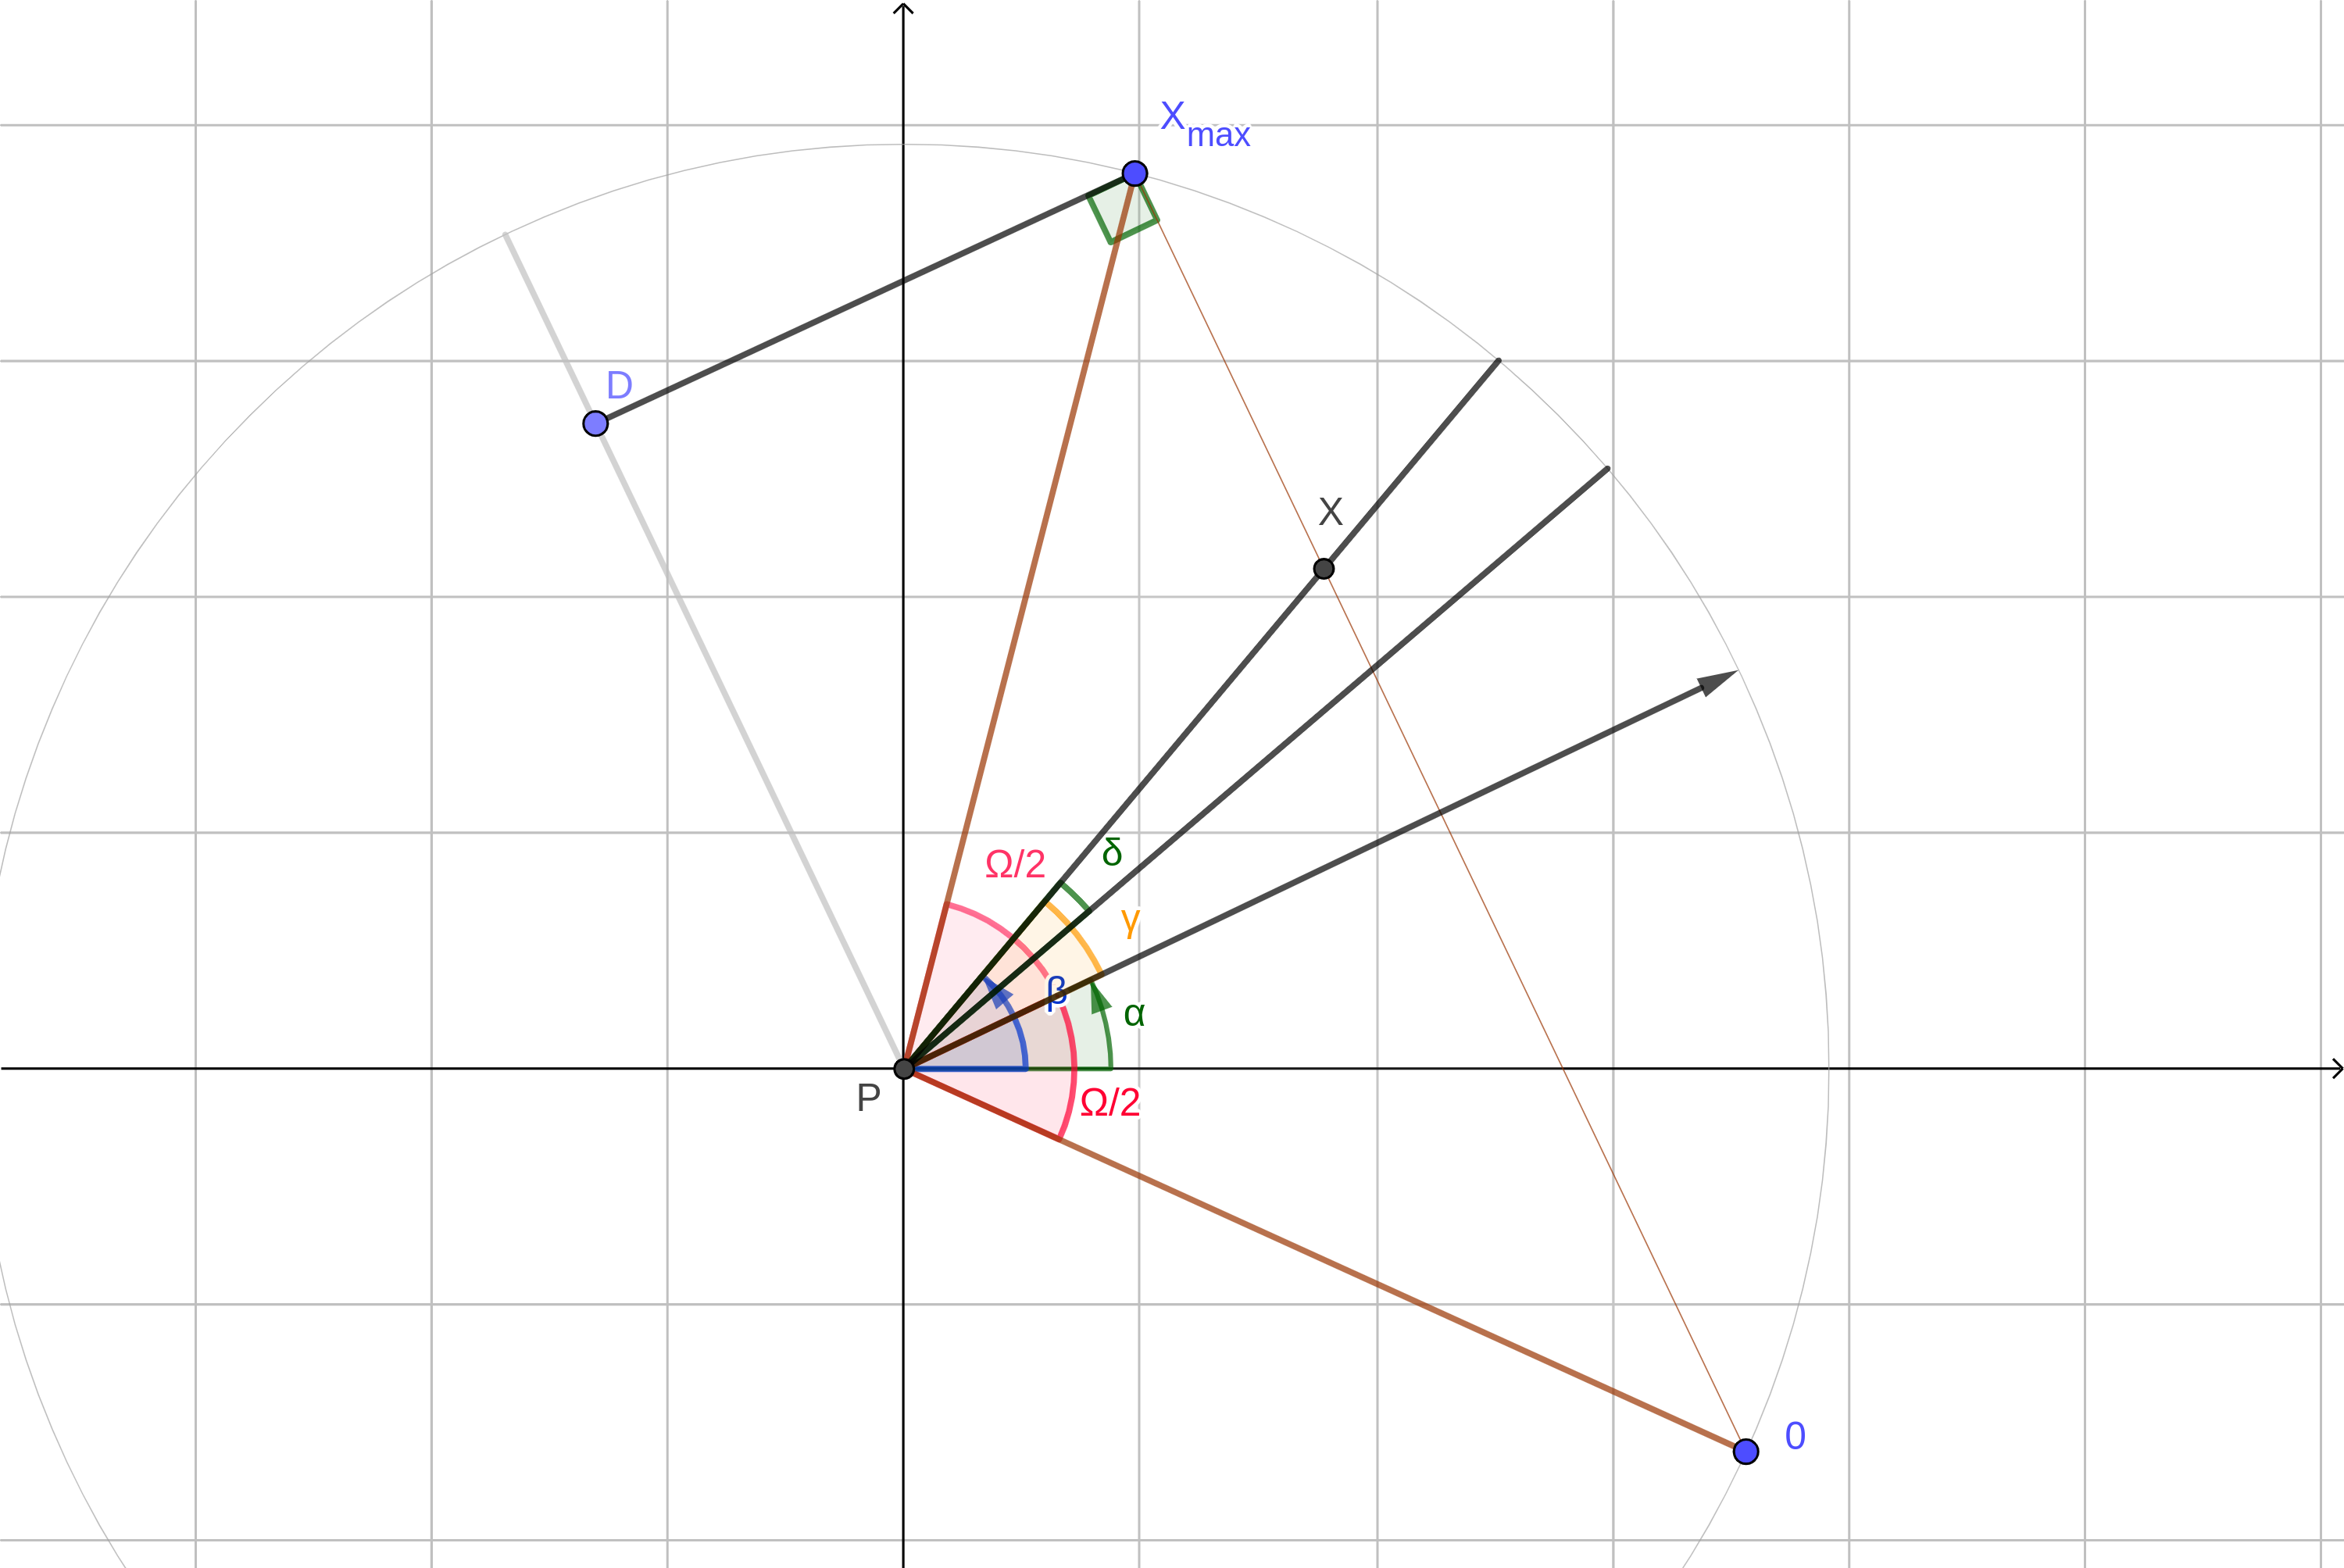
\includegraphics[width=\textwidth]{./images/raycasting.png}
    \caption{Raycasting}
    \label{fig:rays}
\end{figure}

This circle corresponds to the player's maximum view distance ($d$).

It should be noted that half of the cast rays would be on the left side of the player's field of view ($\frac{\Omega}{2}$) and the other half would be on the right side.

Now, we can define the angle between each ray as:

\begin{equation}
    \delta = \frac{\text{Vertical field of view}}{\text{Rays casted}}
\end{equation}

We are going to construct the view of the player by drawing a slice of the view for each ray. The rays would be equally spaced (suspending the angle $\gamma$ at the player) starting from point $O$ till the $X_{max}$.

We'll calculate $X_{max}$ (distance taken from $O$) by using the following formula:

\begin{equation}
    X_{max} = 2 d \sin\frac{\Omega}{2}
\end{equation}

So, the distance $X$ for any ray at angle $\beta$ would be:

\begin{equation}
    X = d \cos\frac{\Omega}{2} \tan\beta
\end{equation}

Now, we can calculate the width of the slice ($W$) for each ray as:

\begin{equation}
    W = \frac{X_{max}}{2} + d \cos\frac{\Omega}{2} (\tan\beta - \tan(\beta - \delta))
\end{equation}

\newpage

